\chapter{提案手法}
本章では提案する手法の詳細について説明する.
まず,提案手法全体の概要を示し,前処理の具体的な手法や分類に使用する機械学習の手法について解説する.

%TODO 分割
\section{提案手法の概要}
\begin{figure}[ht]
  \begin{center}
    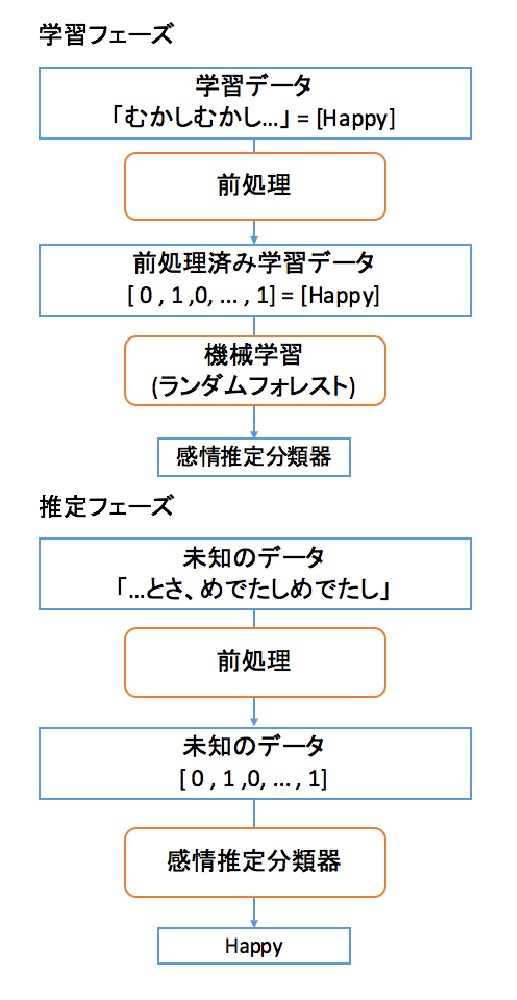
\includegraphics[clip,width=10.0cm]{fig/method-2.eps}
    \caption{提案手法の概要}
    \label{fig:method}
  \end{center}
\end{figure}

提案手法の概要を図\ref{fig:method}に示す.
本手法では,物語中のすべての文に対し文中に含まれる単語の出現を手がかりに朗読に最も適切もしくは自然と感じる感情を推定する.
感情のクラスはNormal,Happy,Sad,Angryの4種類とした.
まず,学習データとして各文に,それぞれ適切と思われる感情を人手で割り当てたものを用意する.
これに対し前処理を行いランダムフォレストを用いて学習を行う.
そして未知の入力文が与えられた場合に,感情クラスの1つを自動的に推定する他クラス分類を行うのが本手法である.

\section{前処理}

\begin{figure}[ht]
  \begin{center}
    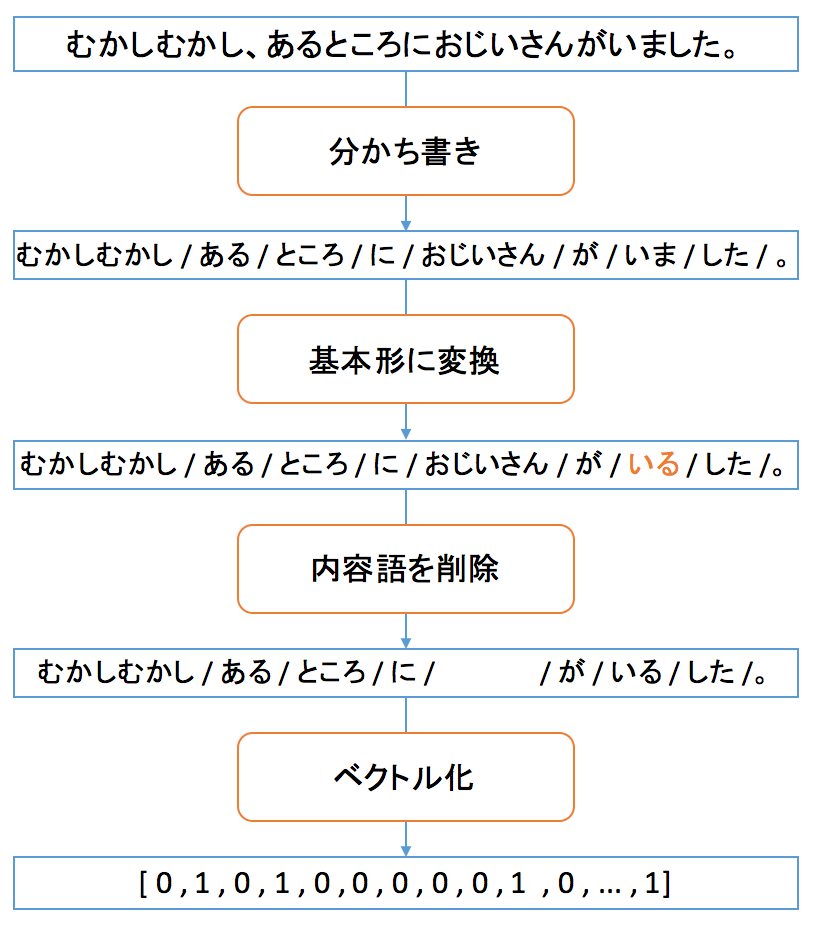
\includegraphics[clip,width=13.0cm]{fig/method.eps}
    \caption{前処理の手順}
    \label{fig:pre}
  \end{center}
\end{figure}

機械学習で
前処理の手法を順に追って説明する.
その概要を図\ref{fig:pre}に示す.


\subsection{文の分割}\label{subsec:divide}
本手法では文単位で感情の推定を行う.
それゆえ,物語の文章を文に分ける必要がある.
意味内容を解読しそれにしたがって分割した方が自然な読み上げが可能になる可能性はあるが,朗読システムの構築を考えると単純な分割が好ましいと判断した.
基本的に,句点で文章を分ける.
カギ括弧で囲まれた箇所はそれを一文とし,その前後の文もそれぞれ一文とする.
%TODO 図で文分割を説明

\subsection{形態素解析}
次に文ごとに形態素解析を行う.
形態素解析とは文法的な情報の注記の無い自然言語の文から,文法や辞書と呼ばれる単語の品詞等の情報にもとづき,言語で意味を持つ最小単位である形態素の列に分割し,それぞれの形態素の品詞等を判別する作業である.
本手法では次節以降で述べる分かち書きと機能語の削除に形態素解析で得られた情報を用いる.

\subsection{分かち書き}
次に分かち書きを行う.
分かち書きとは文を語ごとにわける作業である.
英文の場合は語と語の間に空白(スペース)が入っているが,日本語の場合は入っていないため単純には行えない.
そこで前節の形態素解析の結果を用いて分かち書きを行う.

\subsection{内容語の削除}
本手法は,学習と推定の際に文から内容語(名詞,動詞,形容詞,形容動詞)を取り除き,機能語のみで推定を行う.
なぜならば,未知の物語の感情を推定を目的としているため,学習データが特定の物語に依存していては推定精度が低くとなると考えられるからである.
例えば「鬼」がネガティブに描かれている物語を学習データとして,別の「鬼」がポジティブに描かている物語を推定した場合にネガティブな感情に推定されてしまう恐れがある.
一方,機能後は「しまう」や「ところが」など,朗読時の抑揚などに関係すると考えられる重要な助詞や接続詞を含む.
したがって,内容語を排除し排除し,機能語のみで推定を行う.
このとき,形態素解析を行った結果を用いて,内容語と機能語の判別を行い内容語はデータから削除する.

\subsection{単語列のベクトル化}
分かち書きされた文を機械学習で扱える形式に変換がある.
本手法では,文のベクトル表現の1つであるbag-of-wordsを用いる.
解析で用いるすべての単語文の次元をもつベクトルを用意し文中に単語があれば1とし,なければ0とする.
なお今回は頻度は考慮せず,出現の否かのみを考慮する.

\section{機械学習}
\subsection{ランダムフォレスト}
一般に,入力データに対して,予め定義された複数のクラスから一つを推定する手法として機械学習の教師あり学習が適応できる.
本手法では,その中の手法の1つであるランダムフォレストを用いて機械学習を行う.
波部ら\cite{habe}によると,ランダムフォレストは複数の決定木を用いて森を構成し識別などを行う機械学習アルゴリズムである.
個々の決定木は高い識別性能をもつわけではないが,それらを複数用いてそれぞれの結果を補うことによって高い予測性能を得ることが1つの特徴である.
これは機械学習の分野ではアンサンブル学習と呼ばれており,個々の決定木がアンサンブル学習における弱識別器に相当する.
%TODO エントロピーの説明(数式)


\subsection{グリッドサーチ}
本手法ではより精度を向上させる手法として学習を行う前にグリッドサーチを行う.
グリッドサーチとは学習の際に与えるパラメタそれぞれに対していくつかの値を与え,それらの組み合わせについて学習と交差検証を行いつつ全探索し,最も良いスコアのパラメタを探索する手法である.
本手法で探索するパラメタは表\ref{parameter}の通りである.

\begin{table}[h]
 \centering
  \caption{グリッドサーチで探索したパラメタ}
  \vspace{0.3\baselineskip}
     \scalebox{1}{
  \begin{tabular}{|c|c|} \hline
    パラメタ名&意味\\ \hline \hline
    max\_depth&木の最大の深さ\\ \hline
    n\_estimators&決定木の数\\ \hline
    max\_features&特徴量の最大の数\\ \hline
    criterion&重要度計算の尺度\\ \hline
    min\_sample\_split&葉ノードの最少分割数\\ \hline
    min\_samples\_leaf&葉ノードに用いる特徴量の最小数\\ \hline
  \end{tabular}}
  \label{parameter}
\end{table}


\section{本章のまとめ}
本章では本研究で提案する文に対する感情推定の手法について,文章からベクトルへの変換手法や内容語削除などについて述べた.
次章では,本手法の有効性を示すための実験について説明する.
